% Options for packages loaded elsewhere
\PassOptionsToPackage{unicode}{hyperref}
\PassOptionsToPackage{hyphens}{url}
%
\documentclass[
  ignorenonframetext,
]{beamer}
\usepackage{pgfpages}
\setbeamertemplate{caption}[numbered]
\setbeamertemplate{caption label separator}{: }
\setbeamercolor{caption name}{fg=normal text.fg}
\beamertemplatenavigationsymbolsempty
% Prevent slide breaks in the middle of a paragraph
\widowpenalties 1 10000
\raggedbottom
\setbeamertemplate{part page}{
  \centering
  \begin{beamercolorbox}[sep=16pt,center]{part title}
    \usebeamerfont{part title}\insertpart\par
  \end{beamercolorbox}
}
\setbeamertemplate{section page}{
  \centering
  \begin{beamercolorbox}[sep=12pt,center]{part title}
    \usebeamerfont{section title}\insertsection\par
  \end{beamercolorbox}
}
\setbeamertemplate{subsection page}{
  \centering
  \begin{beamercolorbox}[sep=8pt,center]{part title}
    \usebeamerfont{subsection title}\insertsubsection\par
  \end{beamercolorbox}
}
\AtBeginPart{
  \frame{\partpage}
}
\AtBeginSection{
  \ifbibliography
  \else
    \frame{\sectionpage}
  \fi
}
\AtBeginSubsection{
  \frame{\subsectionpage}
}

\usepackage{amsmath,amssymb}
\usepackage{lmodern}
\usepackage{iftex}
\ifPDFTeX
  \usepackage[T1]{fontenc}
  \usepackage[utf8]{inputenc}
  \usepackage{textcomp} % provide euro and other symbols
\else % if luatex or xetex
  \usepackage{unicode-math}
  \defaultfontfeatures{Scale=MatchLowercase}
  \defaultfontfeatures[\rmfamily]{Ligatures=TeX,Scale=1}
\fi
\usetheme[]{Copenhagen}
% Use upquote if available, for straight quotes in verbatim environments
\IfFileExists{upquote.sty}{\usepackage{upquote}}{}
\IfFileExists{microtype.sty}{% use microtype if available
  \usepackage[]{microtype}
  \UseMicrotypeSet[protrusion]{basicmath} % disable protrusion for tt fonts
}{}
\makeatletter
\@ifundefined{KOMAClassName}{% if non-KOMA class
  \IfFileExists{parskip.sty}{%
    \usepackage{parskip}
  }{% else
    \setlength{\parindent}{0pt}
    \setlength{\parskip}{6pt plus 2pt minus 1pt}}
}{% if KOMA class
  \KOMAoptions{parskip=half}}
\makeatother
\usepackage{xcolor}
\newif\ifbibliography
\setlength{\emergencystretch}{3em} % prevent overfull lines
\setcounter{secnumdepth}{-\maxdimen} % remove section numbering


\providecommand{\tightlist}{%
  \setlength{\itemsep}{0pt}\setlength{\parskip}{0pt}}\usepackage{longtable,booktabs,array}
\usepackage{calc} % for calculating minipage widths
\usepackage{caption}
% Make caption package work with longtable
\makeatletter
\def\fnum@table{\tablename~\thetable}
\makeatother
\usepackage{graphicx}
\makeatletter
\def\maxwidth{\ifdim\Gin@nat@width>\linewidth\linewidth\else\Gin@nat@width\fi}
\def\maxheight{\ifdim\Gin@nat@height>\textheight\textheight\else\Gin@nat@height\fi}
\makeatother
% Scale images if necessary, so that they will not overflow the page
% margins by default, and it is still possible to overwrite the defaults
% using explicit options in \includegraphics[width, height, ...]{}
\setkeys{Gin}{width=\maxwidth,height=\maxheight,keepaspectratio}
% Set default figure placement to htbp
\makeatletter
\def\fps@figure{htbp}
\makeatother

\makeatletter
\makeatother
\makeatletter
\makeatother
\makeatletter
\@ifpackageloaded{caption}{}{\usepackage{caption}}
\AtBeginDocument{%
\ifdefined\contentsname
  \renewcommand*\contentsname{Table of contents}
\else
  \newcommand\contentsname{Table of contents}
\fi
\ifdefined\listfigurename
  \renewcommand*\listfigurename{List of Figures}
\else
  \newcommand\listfigurename{List of Figures}
\fi
\ifdefined\listtablename
  \renewcommand*\listtablename{List of Tables}
\else
  \newcommand\listtablename{List of Tables}
\fi
\ifdefined\figurename
  \renewcommand*\figurename{Figure}
\else
  \newcommand\figurename{Figure}
\fi
\ifdefined\tablename
  \renewcommand*\tablename{Table}
\else
  \newcommand\tablename{Table}
\fi
}
\@ifpackageloaded{float}{}{\usepackage{float}}
\floatstyle{ruled}
\@ifundefined{c@chapter}{\newfloat{codelisting}{h}{lop}}{\newfloat{codelisting}{h}{lop}[chapter]}
\floatname{codelisting}{Listing}
\newcommand*\listoflistings{\listof{codelisting}{List of Listings}}
\makeatother
\makeatletter
\@ifpackageloaded{caption}{}{\usepackage{caption}}
\@ifpackageloaded{subcaption}{}{\usepackage{subcaption}}
\makeatother
\makeatletter
\@ifpackageloaded{tcolorbox}{}{\usepackage[many]{tcolorbox}}
\makeatother
\makeatletter
\@ifundefined{shadecolor}{\definecolor{shadecolor}{rgb}{.97, .97, .97}}
\makeatother
\makeatletter
\makeatother
\ifLuaTeX
  \usepackage{selnolig}  % disable illegal ligatures
\fi
\IfFileExists{bookmark.sty}{\usepackage{bookmark}}{\usepackage{hyperref}}
\IfFileExists{xurl.sty}{\usepackage{xurl}}{} % add URL line breaks if available
\urlstyle{same} % disable monospaced font for URLs
\hypersetup{
  pdftitle={Pakistan Health Infrastructure Outlook},
  pdfauthor={Stat Devs},
  hidelinks,
  pdfcreator={LaTeX via pandoc}}

\title{Pakistan Health Infrastructure Outlook}
\author{Stat Devs}
\date{}

\begin{document}
\frame{\titlepage}
\ifdefined\Shaded\renewenvironment{Shaded}{\begin{tcolorbox}[breakable, frame hidden, enhanced, sharp corners, borderline west={3pt}{0pt}{shadecolor}, boxrule=0pt, interior hidden]}{\end{tcolorbox}}\fi

\begin{frame}{Introduction to Exploratory Sunday}
\protect\hypertarget{introduction-to-exploratory-sunday}{}
\begin{itemize}
\item
  Exploratory Sunday is a social awareness campaign initiated by
  StatDevs.
\item
  Every Sunday, we post weekly statistics and visualizations
  concentrating on Pakistan's demographic, healthcare and socio-economic
  indicators.
\item
  The aim of this compaign is to raise awareness to masses about how
  Pakistan's conditions stack up against Sustainable Development Goals.
\item
  These posts are made using Open Source data sets such as
  PDHS(2017-18), PSLM(2019-20), Pakistan Census (2017) data.
\end{itemize}
\end{frame}

\begin{frame}{How is Pakistan demographically distributed?}
\protect\hypertarget{how-is-pakistan-demographically-distributed}{}
\begin{figure}

{\centering 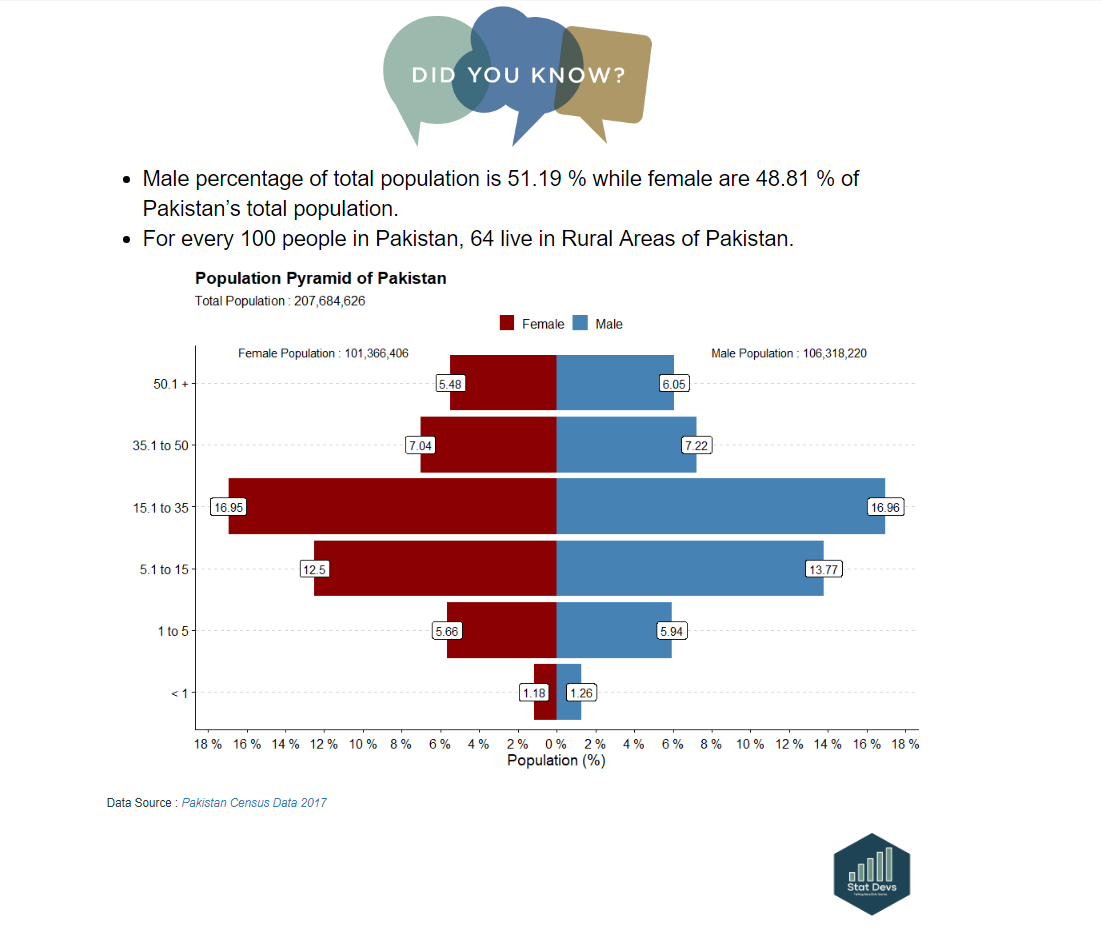
\includegraphics{Demographics-Final.png}

}

\end{figure}
\end{frame}

\begin{frame}{Pakistan sits in Lower Income group in Global Health
Spending}
\protect\hypertarget{pakistan-sits-in-lower-income-group-in-global-health-spending}{}
\begin{figure}

{\centering 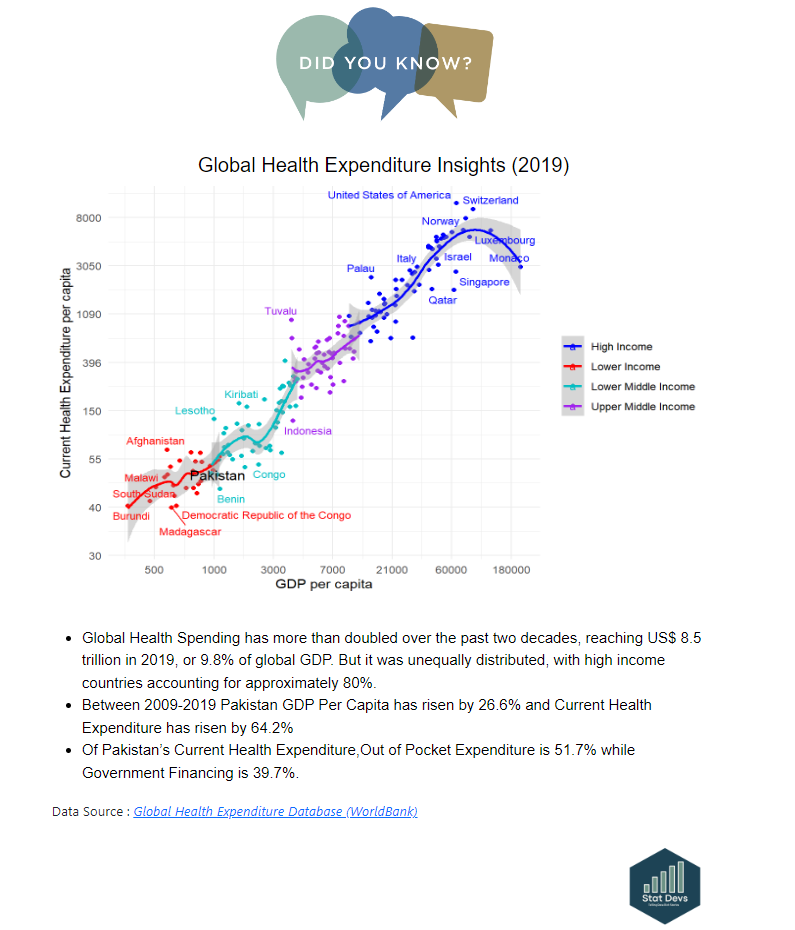
\includegraphics{Final Global Health.png}

}

\end{figure}
\end{frame}

\begin{frame}{On average 52\% of health financing is Out of Pocket
Expenditure in Pakistan}
\protect\hypertarget{on-average-52-of-health-financing-is-out-of-pocket-expenditure-in-pakistan}{}
\begin{figure}

{\centering 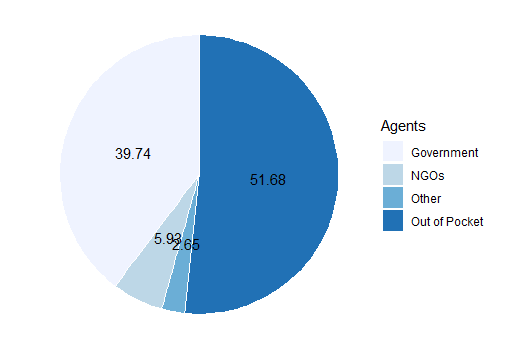
\includegraphics{health-financing.png}

}

\end{figure}
\end{frame}

\begin{frame}{What is Pakistan's Health Infrastruce Outlook?}
\protect\hypertarget{what-is-pakistans-health-infrastruce-outlook}{}
\begin{figure}

{\centering 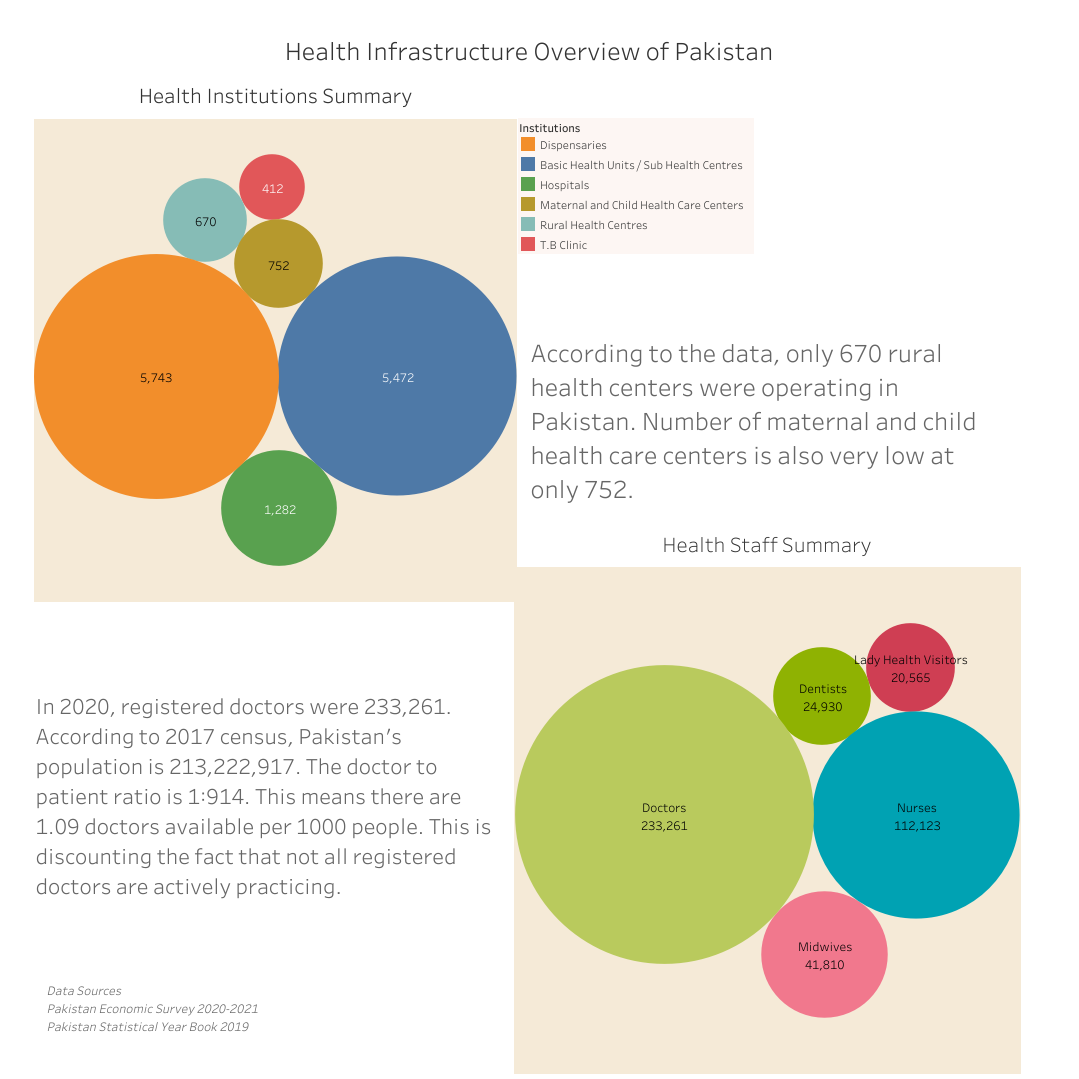
\includegraphics{health-infrastructure.png}

}

\end{figure}
\end{frame}

\begin{frame}{More RHCs \& BHUs are needed to cover the health disparity
in Pakistan}
\protect\hypertarget{more-rhcs-bhus-are-needed-to-cover-the-health-disparity-in-pakistan}{}
\begin{figure}

{\centering 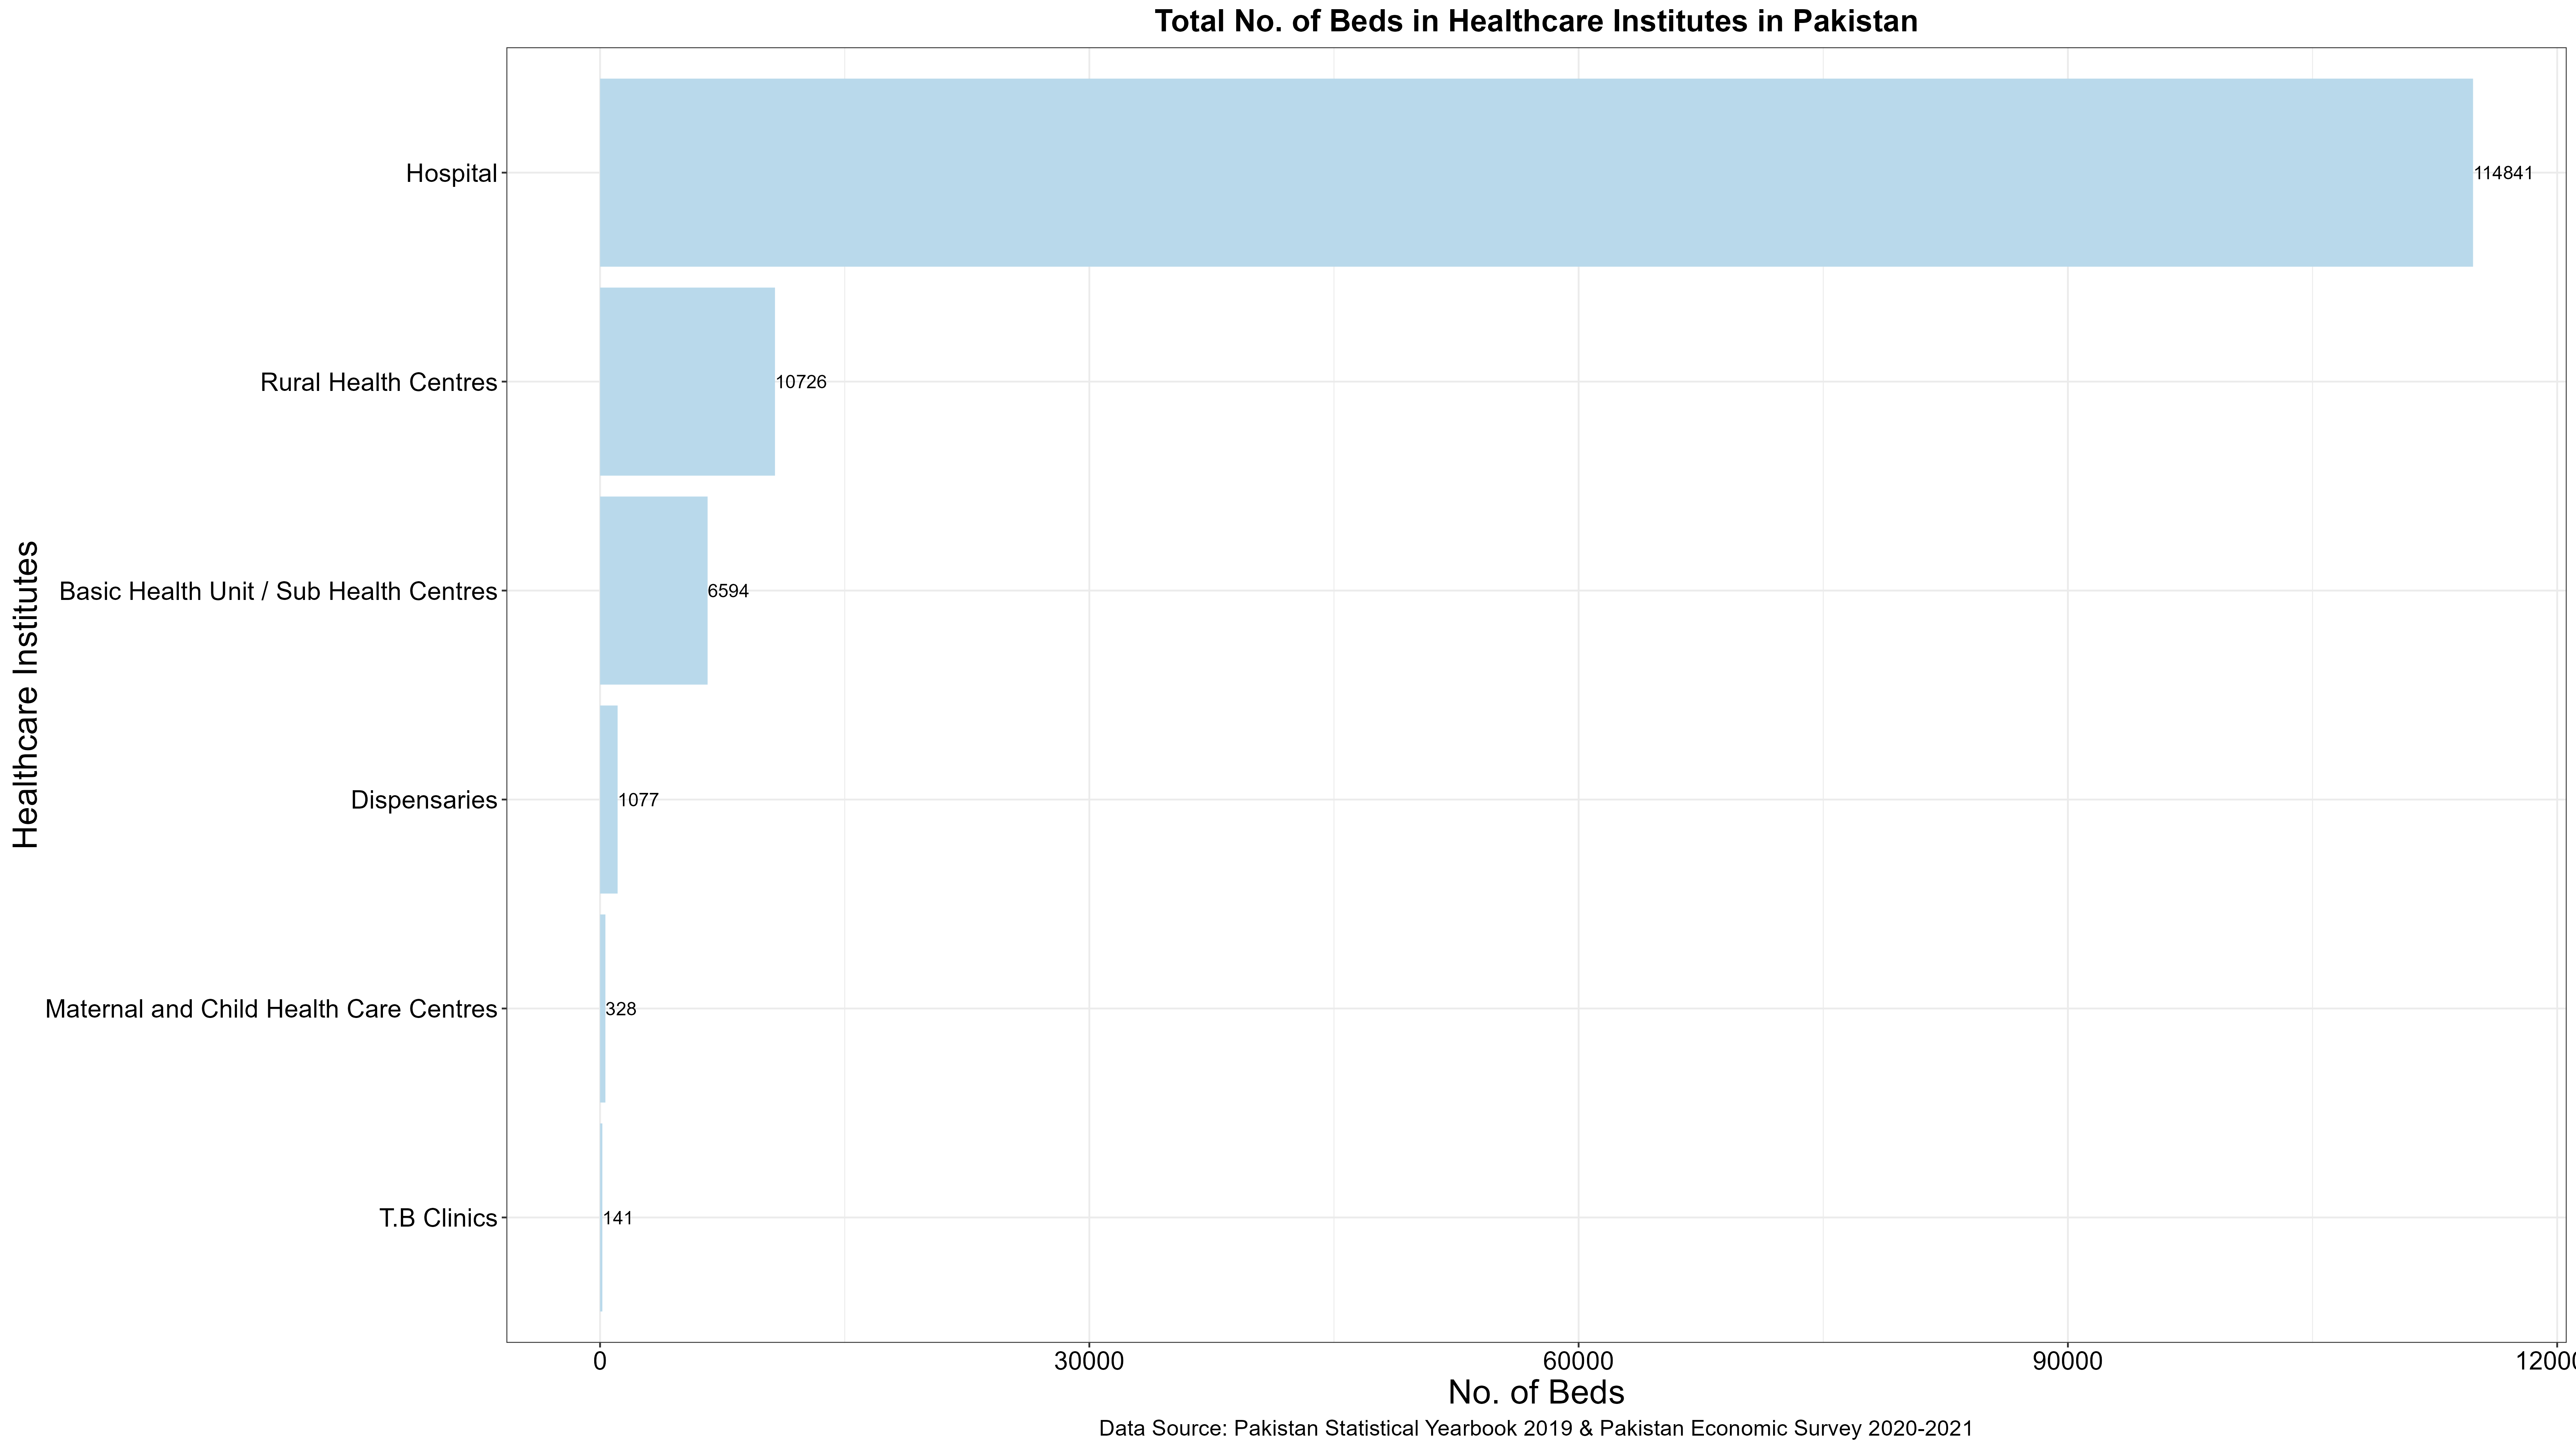
\includegraphics{beds.png}

}

\end{figure}
\end{frame}

\begin{frame}{Supply of Health Infrastructure is low in Balochistan}
\protect\hypertarget{supply-of-health-infrastructure-is-low-in-balochistan}{}
\begin{figure}

{\centering 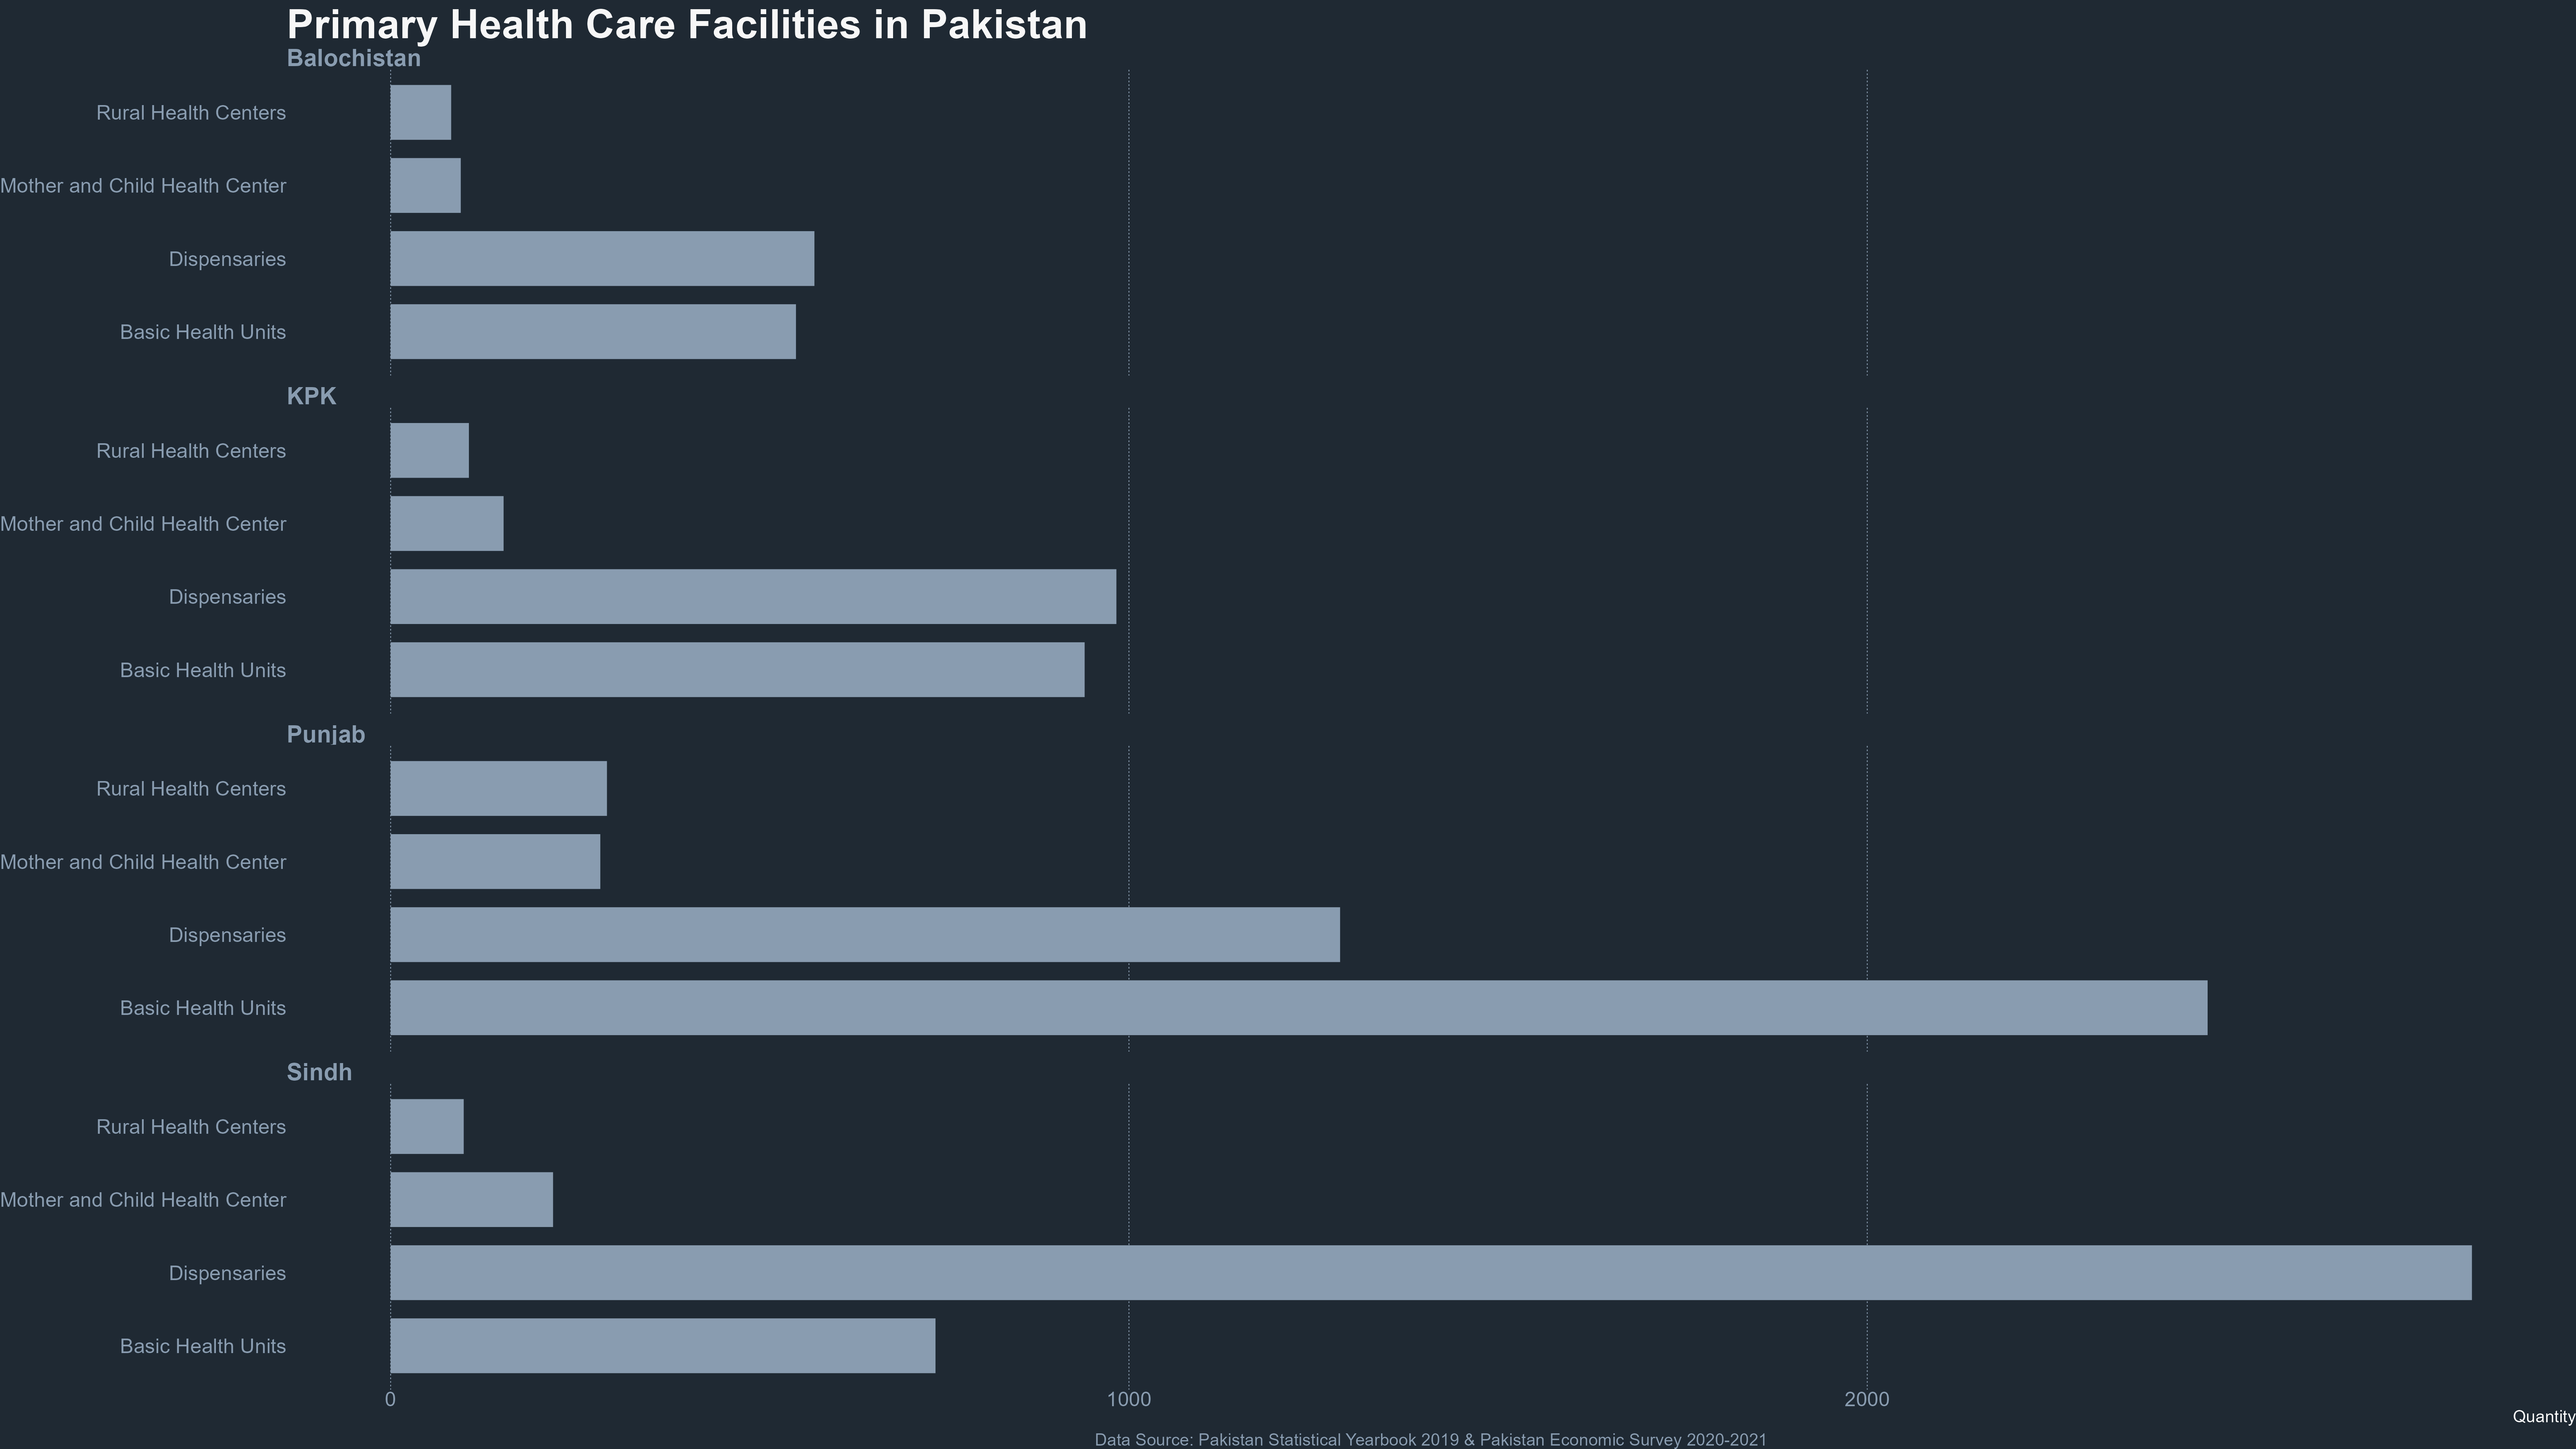
\includegraphics{primary_health_facilities.png}

}

\end{figure}
\end{frame}

\begin{frame}{Balochistan lacks prenatal consultation by health
specialist}
\protect\hypertarget{balochistan-lacks-prenatal-consultation-by-health-specialist}{}
\begin{figure}

{\centering 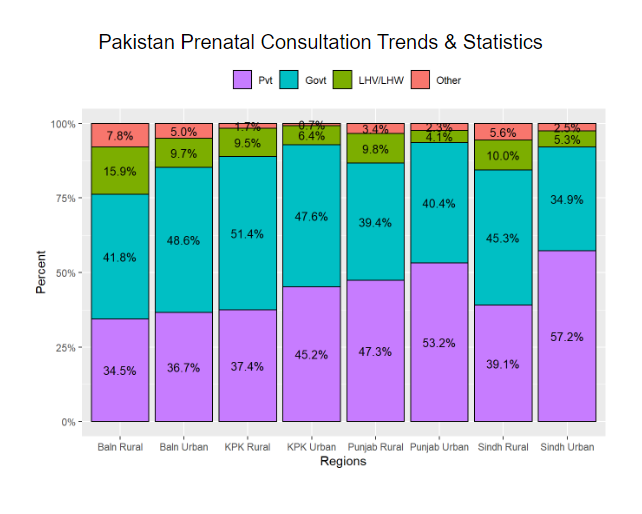
\includegraphics{Prenatal-Statistics-crop.png}

}

\end{figure}
\end{frame}

\begin{frame}{Call to Action}
\protect\hypertarget{call-to-action}{}
\begin{itemize}
\item
  Pakistan's healthcare system relies predominantly on Out-of Pocket
  financing.
\item
  Spatial disparities in access to basic to health necessities has
  widened in Pakistan.
\item
  The burden of out-of-pocket expenditure is much greater for poor
  households than rich ones.
\item
  Ensuring implementation and monitoring the correctness of the laws by
  health system governance can help reduce OOP payments and can improve
  Pakistan Health Infrastructure.
\end{itemize}
\end{frame}



% Template basé sur le code d'E. Quinton (INRAE)

\thispagestyle{empty}

\newgeometry{left=2cm,bottom=0.1cm}

\begin{center}

\color{statdevs}

\vspace*{10cm}


\includegraphics[height=0.6cm]{quarto-statdevs-template/images/fleche-titre.png}\par

\sffamily
Stat Devs -- Research Unit\\
Address\\
86-C, 4th Floor, 11th Commercial Street, Kh-e-Ittehad, \\
Phase-2 Extn, DHA, Karachi 75500 \\
+923368446579\\
+923312803120\par\bigskip

%Join Us On :\\

\includegraphics{quarto-statdevs-template/images/social-media.png}\par\bigskip

\vspace*{2cm}

%{\bfseries Institut national de recherche pour\\
%l'agriculture, l'alimentation et l'environnement}
\par\bigskip


\includegraphics[width=5cm]{quarto-statdevs-template/images/Final-Logo.png}\par

\end{center}

\restoregeometry

\end{document}
